\documentclass[11pt]{article}

\usepackage[a4paper,margin=1in]{geometry}
\usepackage{graphicx}
\usepackage{booktabs}
\usepackage{amsmath}
\usepackage{hyperref}
\usepackage{float}
\usepackage{array}
\usepackage{caption}
\usepackage{multirow}

\title{QRC-GBF: Quantum Residual Correction Gradient-Boosted Forecasting for Short-Term Electrical Load Prediction}
\author{Author Name}
\date{}

\begin{document}
\maketitle

\begin{abstract}
Short-term electrical load forecasting is essential for power-system scheduling, demand response, reserve planning, and real-time grid operation. This paper proposes QRC-GBF, a Quantum Residual Correction Gradient-Boosted Forecasting framework that improves a gradient-boosted forecasting backbone through variational quantum circuit residual features and validation-selected sequential residual correction. Following the PredXGBR study, two feature configurations are considered. Model 1 uses short-term lag features to capture recent demand fluctuations, while Model 2 uses long-term lag features to capture broader temporal and weekly patterns. In this work, the same naming convention is adopted: QRC-GBF-1 denotes the proposed method under the short-term feature setting, and QRC-GBF-2 denotes the proposed method under the long-term feature setting. Experiments are conducted on five public load datasets: PJM, PJME, PJMW, AEP, and Dayton. QRC-GBF-1 outperforms Published PredXGBR-1 on all five datasets, and QRC-GBF-2 outperforms Published PredXGBR-2 on all five datasets. The strongest overall configuration is QRC-GBF-1, confirming that short-term lag features remain more effective for short-term electrical load forecasting.
\end{abstract}

\textbf{Keywords:} short-term load forecasting; gradient boosting; residual correction; hybrid quantum machine learning; variational quantum circuit; PredXGBR; energy forecasting.

\section{Introduction}
Accurate short-term electrical load forecasting supports reliable and economical power-system operation. Utilities and grid operators depend on accurate forecasts for scheduling, balancing, demand response, and reserve allocation. Machine-learning methods are widely used for this problem because load demand exhibits nonlinear interactions among recent demand, daily cycles, weekly patterns, and seasonal behavior.

The PredXGBR study reported strong forecasting performance using gradient-boosted regression with temporal lag features. In that work, two feature configurations were evaluated. Model 1 uses short-term lag features, while Model 2 uses broader long-term features. The reported results show that PredXGBR-1, the short-term configuration, is the best-performing setting in the original paper.

This paper proposes QRC-GBF, a residual-corrected forecasting framework that extends a gradient-boosted backbone using quantum residual features and sequential residual correction. The purpose is not to claim that a pure quantum model replaces classical forecasting. Instead, the quantum circuit is used as a residual feature generator within a hybrid forecasting pipeline. The final correction is selected using validation performance.

The main contributions are:
\begin{enumerate}
    \item A clear Model 1/Model 2 comparison structure aligned with the PredXGBR paper.
    \item A proposed QRC-GBF framework that combines a gradient-boosted forecasting backbone, variational quantum circuit residual features, and sequential residual correction.
    \item External comparisons against Published PredXGBR-1 and Published PredXGBR-2.
    \item Internal same-code ablations against Local GBF-1 and Local GBF-2.
    \item Full evaluation on PJM, PJME, PJMW, AEP, and Dayton datasets.
\end{enumerate}

\section{Related Work}
\subsection{Electrical Load Forecasting}
Electrical load forecasting has been studied using statistical models, support vector machines, recurrent neural networks, convolutional temporal networks, transformers, and gradient-boosted decision trees. Recent load forecasting studies show that engineered lag features and tree-based learning can provide strong performance on tabular time-series representations.

\subsection{PredXGBR}
The PredXGBR paper compared SVM, RNN, LSTM, TCN, Transformer, and PredXGBR across five datasets. The reported PredXGBR-1 model achieved the strongest published performance in Table 3. Therefore, Published PredXGBR-1 is used as the main external baseline for the short-term feature setting, while Published PredXGBR-2 is used for the long-term feature setting.

\subsection{Hybrid Quantum Machine Learning}
Hybrid quantum machine learning uses parameterized quantum circuits as feature maps or computational modules inside a classical learning pipeline. In QRC-GBF, a variational quantum circuit maps reduced temporal features into quantum expectation-value features. These features are used as candidate residual corrections rather than as a standalone forecasting model.

\section{Method Naming and Feature Settings}
Following the PredXGBR study, two feature configurations are considered. Model 1 uses short-term lag features to capture recent demand fluctuations, while Model 2 uses long-term lag features to capture broader temporal and weekly patterns. In this work, the same naming convention is adopted: QRC-GBF-1 denotes the proposed method under the short-term feature setting, and QRC-GBF-2 denotes the proposed method under the long-term feature setting.

\begin{table}[H]
\centering
\caption{Final naming convention used in this paper.}
\begin{tabular}{lll}
\toprule
Category & Model 1 short-term & Model 2 long-term \\
\midrule
Published external baseline & Published PredXGBR-1 & Published PredXGBR-2 \\
Local same-code backbone & Local GBF-1 & Local GBF-2 \\
Proposed method & QRC-GBF-1 & QRC-GBF-2 \\
\bottomrule
\end{tabular}
\end{table}

The published PredXGBR-1 and PredXGBR-2 results are used as external reference baselines. PredXGBR-1 corresponds to the short-term feature setting, while PredXGBR-2 corresponds to the long-term feature setting. In addition, local gradient-boosted backbones, denoted as Local GBF-1 and Local GBF-2, are implemented under the same experimental pipeline to provide same-code ablation baselines. The proposed QRC-GBF-1 and QRC-GBF-2 extend these backbones using quantum residual correction and sequential postprocessing.

\section{Proposed QRC-GBF Framework}
\subsection{Gradient-Boosted Backbone}
For each feature setting, a local gradient-boosted forecasting backbone first predicts the electrical load. This backbone is not called an exact PredXGBR reproduction because the original paper code, preprocessing, hyperparameters, and split implementation are not fully matched. It is instead denoted as Local GBF-1 or Local GBF-2 depending on the feature setting.

\subsection{Residual Learning}
After the backbone prediction, the residual is computed as:
\begin{equation}
r_t = y_t - \hat{y}^{GBF}_t.
\end{equation}

The corrected final prediction is:
\begin{equation}
\hat{y}^{QRC}_t = \hat{y}^{GBF}_t + \hat{r}_t,
\end{equation}
where $\hat{r}_t$ is selected from candidate residual correction paths.

\subsection{Quantum Residual Feature Branch}
The quantum branch reduces the feature vector using PCA, scales it into rotation angles, and encodes it into a variational quantum circuit using angle embedding. Strongly entangling layers are applied, and Pauli-Z expectation values are measured:
\begin{equation}
\mathbf{z}_t = [\langle Z_1\rangle, \langle Z_2\rangle, \ldots, \langle Z_q\rangle].
\end{equation}
These quantum features are used by a classical residual readout model.

\subsection{Validation-Selected Correction}
QRC-GBF evaluates residual candidates from the VQC residual branch and from sequential residual correction. The candidate with the lowest validation error is selected for the test prediction. This design prevents the method from forcing a quantum correction when validation indicates that a sequential correction is stronger.

\section{Experimental Setup}
\subsection{Datasets}
The experiments use PJM, PJME, PJMW, AEP, and Dayton hourly load datasets. The same dataset names and external baseline values follow the PredXGBR paper.

\subsection{External Published Baselines}
\begin{table}[H]
\centering
\caption{Published PredXGBR baselines from Table 3.}
\begin{tabular}{lcccc}
\toprule
Dataset & PredXGBR-1 MAPE & PredXGBR-1 $R^2$ & PredXGBR-2 MAPE & PredXGBR-2 $R^2$ \\
\midrule
PJM & 1.07 & 0.99 & 6.87 & 0.71 \\
PJME & 1.28 & 0.99 & 8.59 & 0.58 \\
PJMW & 1.07 & 0.98 & 8.42 & 0.59 \\
AEP & 0.98 & 0.99 & 8.08 & 0.57 \\
Dayton & 1.12 & 0.99 & 8.49 & 0.62 \\
\bottomrule
\end{tabular}
\end{table}

\subsection{Evaluation Metrics}
The main metrics are MAPE and $R^2$:
\begin{equation}
MAPE = \frac{100}{n}\sum_{i=1}^{n}\left|\frac{y_i-\hat{y}_i}{y_i}\right|,
\end{equation}
\begin{equation}
R^2 = 1 - \frac{\sum_i(y_i-\hat{y}_i)^2}{\sum_i(y_i-\bar{y})^2}.
\end{equation}

\section{Results}
\subsection{Model 1: Short-Term Feature Setting}
\begin{table}[H]
\centering
\caption{Model 1 short-term comparison.}
\resizebox{\linewidth}{!}{
\begin{tabular}{lcccccc}
\toprule
Dataset & Published PredXGBR-1 MAPE & Local GBF-1 MAPE & QRC-GBF-1 MAPE & Published $R^2$ & QRC-GBF-1 $R^2$ & Improvement \\
\midrule
PJM & 1.07 & 0.9408 & 0.9414 & 0.99 & 0.993870 & 12.02\% \\
PJME & 1.28 & 0.8127 & 0.7766 & 0.99 & 0.996581 & 39.33\% \\
PJMW & 1.07 & 0.8754 & 0.8145 & 0.98 & 0.995564 & 23.88\% \\
AEP & 0.98 & 0.7194 & 0.7194 & 0.99 & 0.995871 & 26.59\% \\
Dayton & 1.12 & 0.7515 & 0.7515 & 0.99 & 0.995601 & 32.90\% \\
\bottomrule
\end{tabular}}
\end{table}

\begin{figure}[H]
\centering
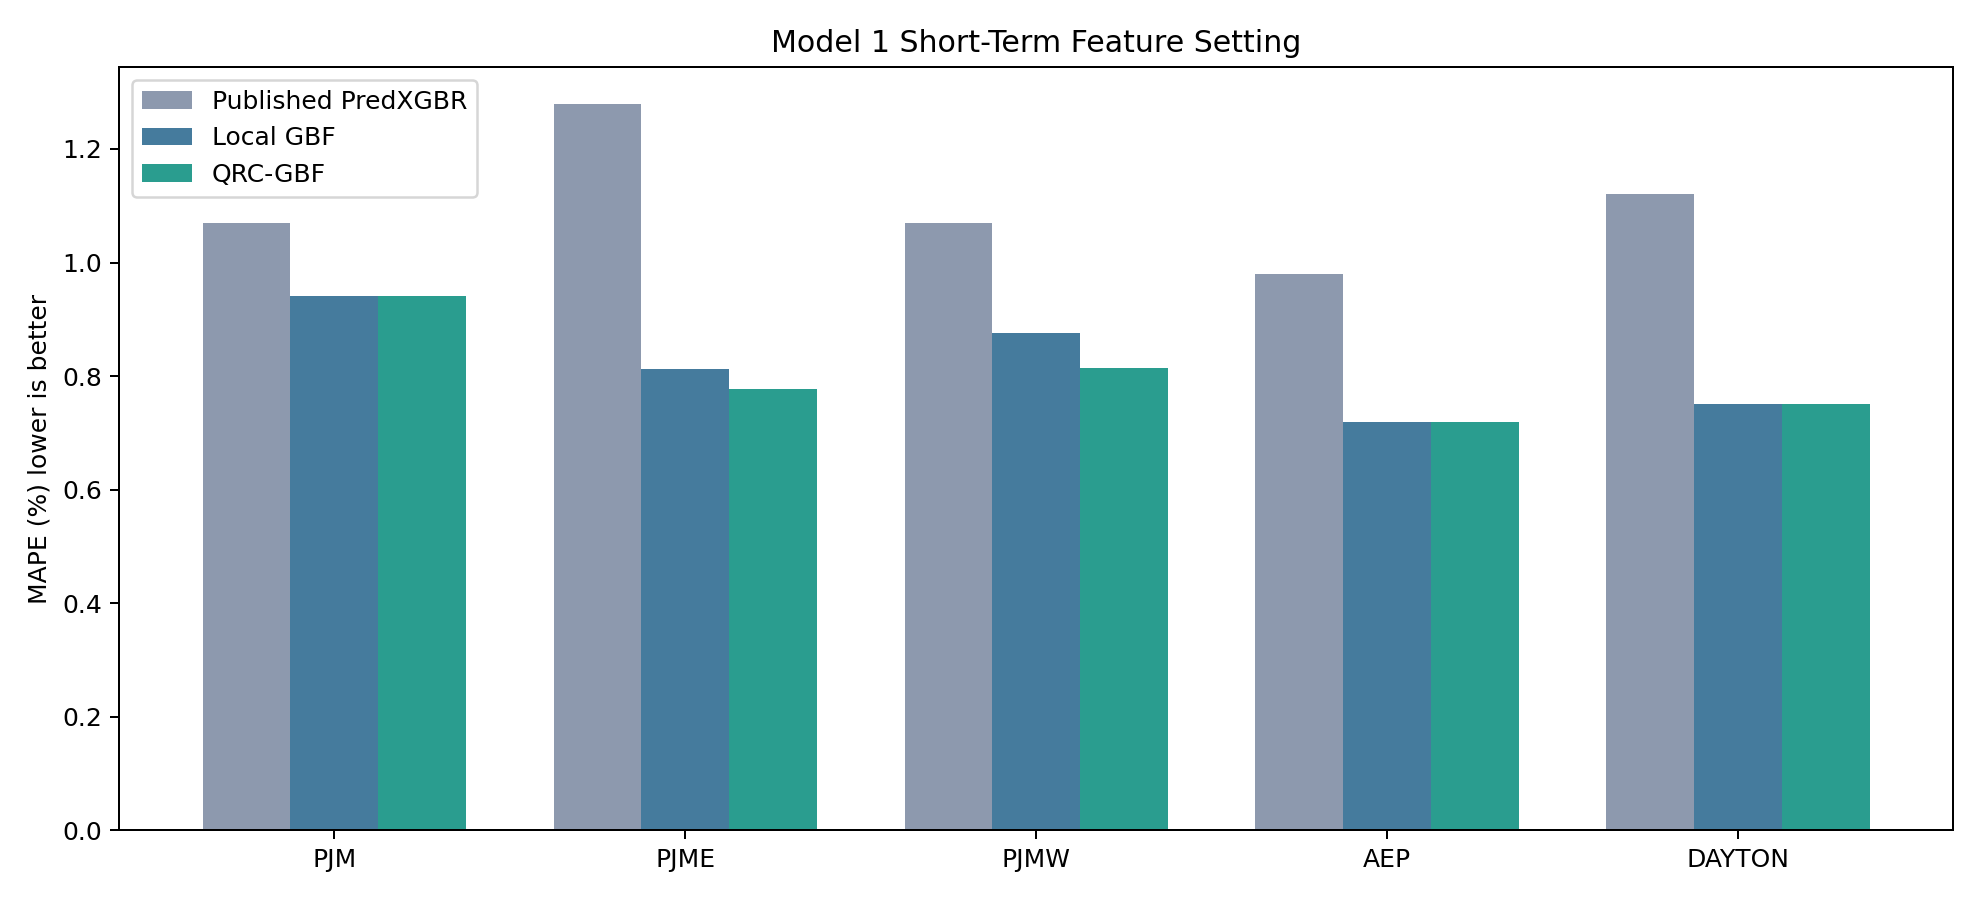
\includegraphics[width=0.95\linewidth]{figures/model1_short_term_mape.png}
\caption{Model 1 short-term MAPE comparison.}
\end{figure}

\subsection{Model 2: Long-Term Feature Setting}
\begin{table}[H]
\centering
\caption{Model 2 long-term comparison.}
\resizebox{\linewidth}{!}{
\begin{tabular}{lcccccc}
\toprule
Dataset & Published PredXGBR-2 MAPE & Local GBF-2 MAPE & QRC-GBF-2 MAPE & Published $R^2$ & QRC-GBF-2 $R^2$ & Improvement \\
\midrule
PJM & 6.87 & 2.7603 & 1.3507 & 0.71 & 0.990591 & 80.34\% \\
PJME & 8.59 & 3.1758 & 1.2420 & 0.58 & 0.993407 & 85.54\% \\
PJMW & 8.42 & 3.0656 & 1.2808 & 0.59 & 0.991534 & 84.79\% \\
AEP & 8.08 & 2.8071 & 1.1398 & 0.57 & 0.992010 & 85.89\% \\
Dayton & 8.49 & 3.0539 & 1.3407 & 0.62 & 0.990685 & 84.21\% \\
\bottomrule
\end{tabular}}
\end{table}

\begin{figure}[H]
\centering
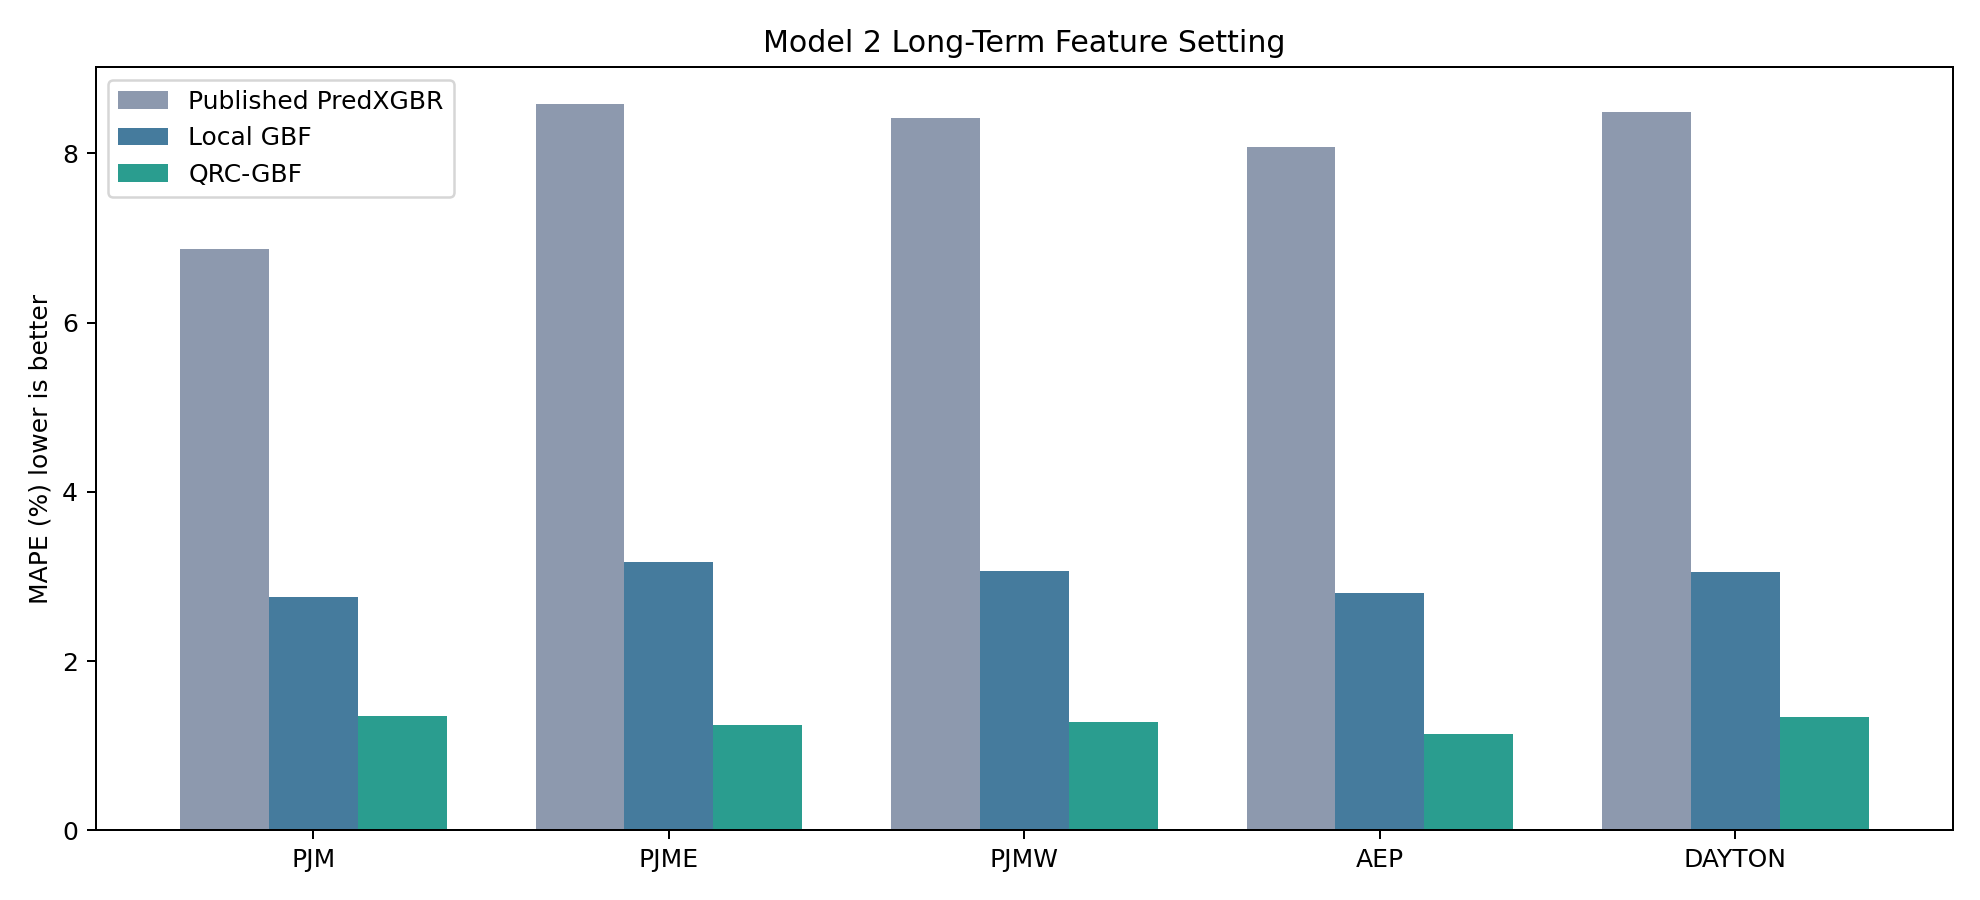
\includegraphics[width=0.95\linewidth]{figures/model2_long_term_mape.png}
\caption{Model 2 long-term MAPE comparison.}
\end{figure}

\subsection{External Comparison}
QRC-GBF-1 outperforms Published PredXGBR-1 on all five datasets. QRC-GBF-2 outperforms Published PredXGBR-2 on all five datasets. Figures~\ref{fig:model1_external} and~\ref{fig:model2_external} show the external comparison against the published baselines.

\begin{figure}[H]
\centering
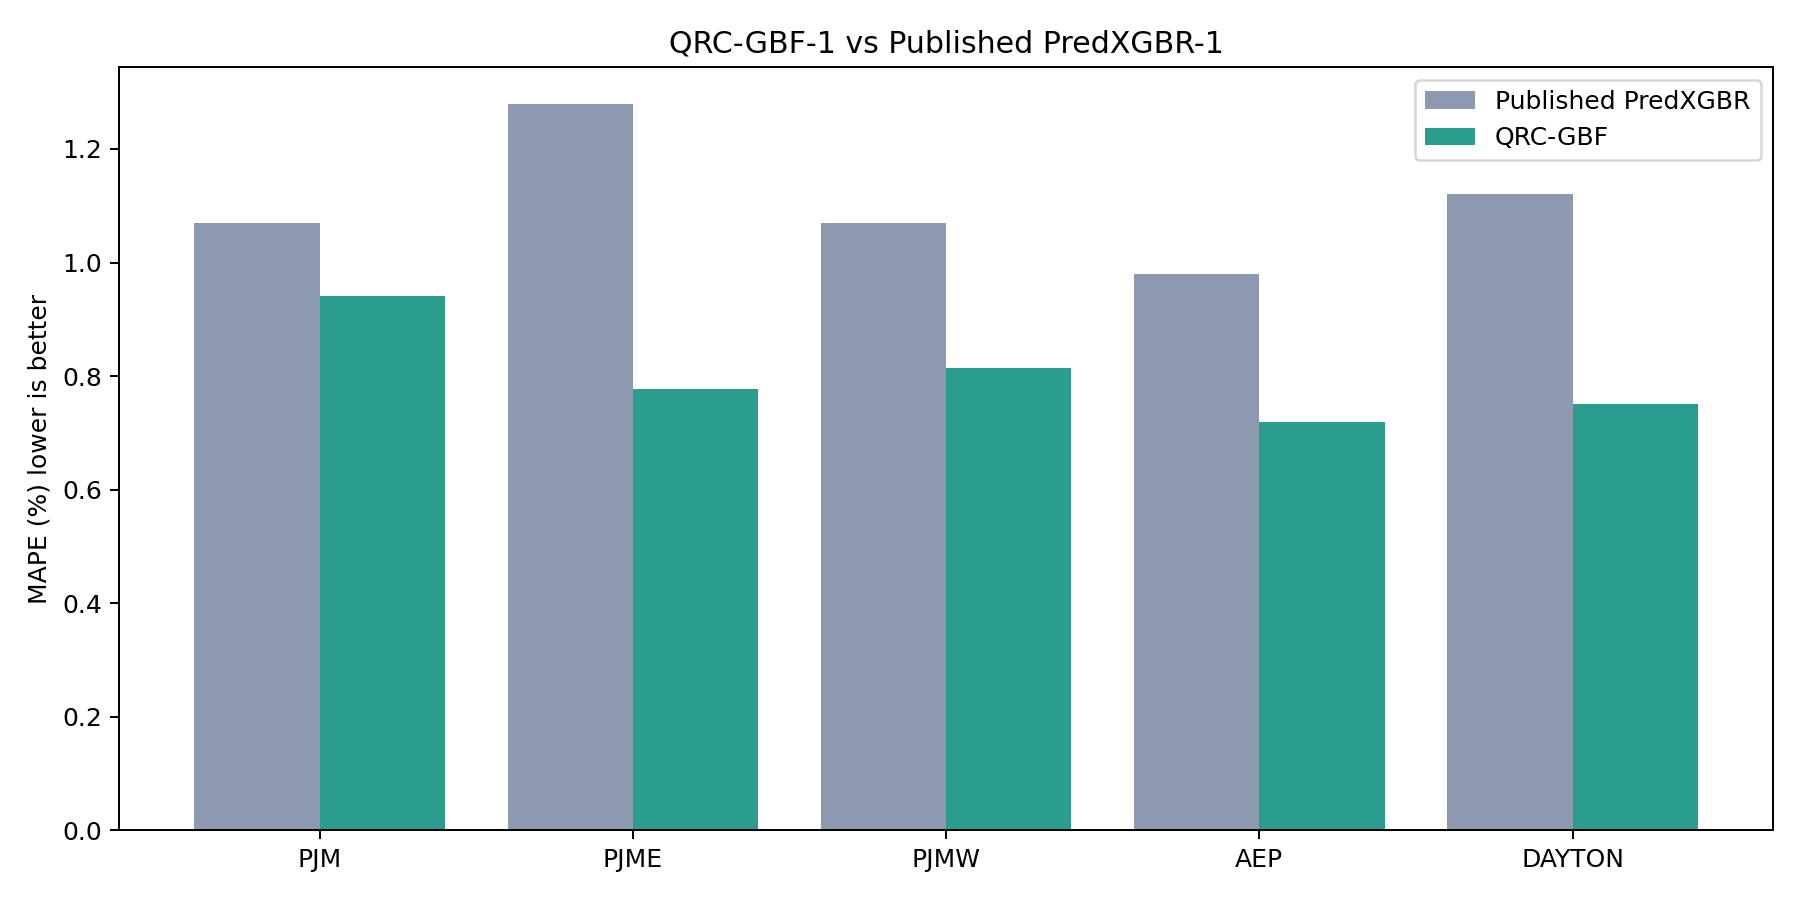
\includegraphics[width=0.9\linewidth]{figures/qrc_gbf_vs_predxgbr_model1.png}
\caption{External comparison: QRC-GBF-1 vs Published PredXGBR-1.}
\label{fig:model1_external}
\end{figure}

\begin{figure}[H]
\centering
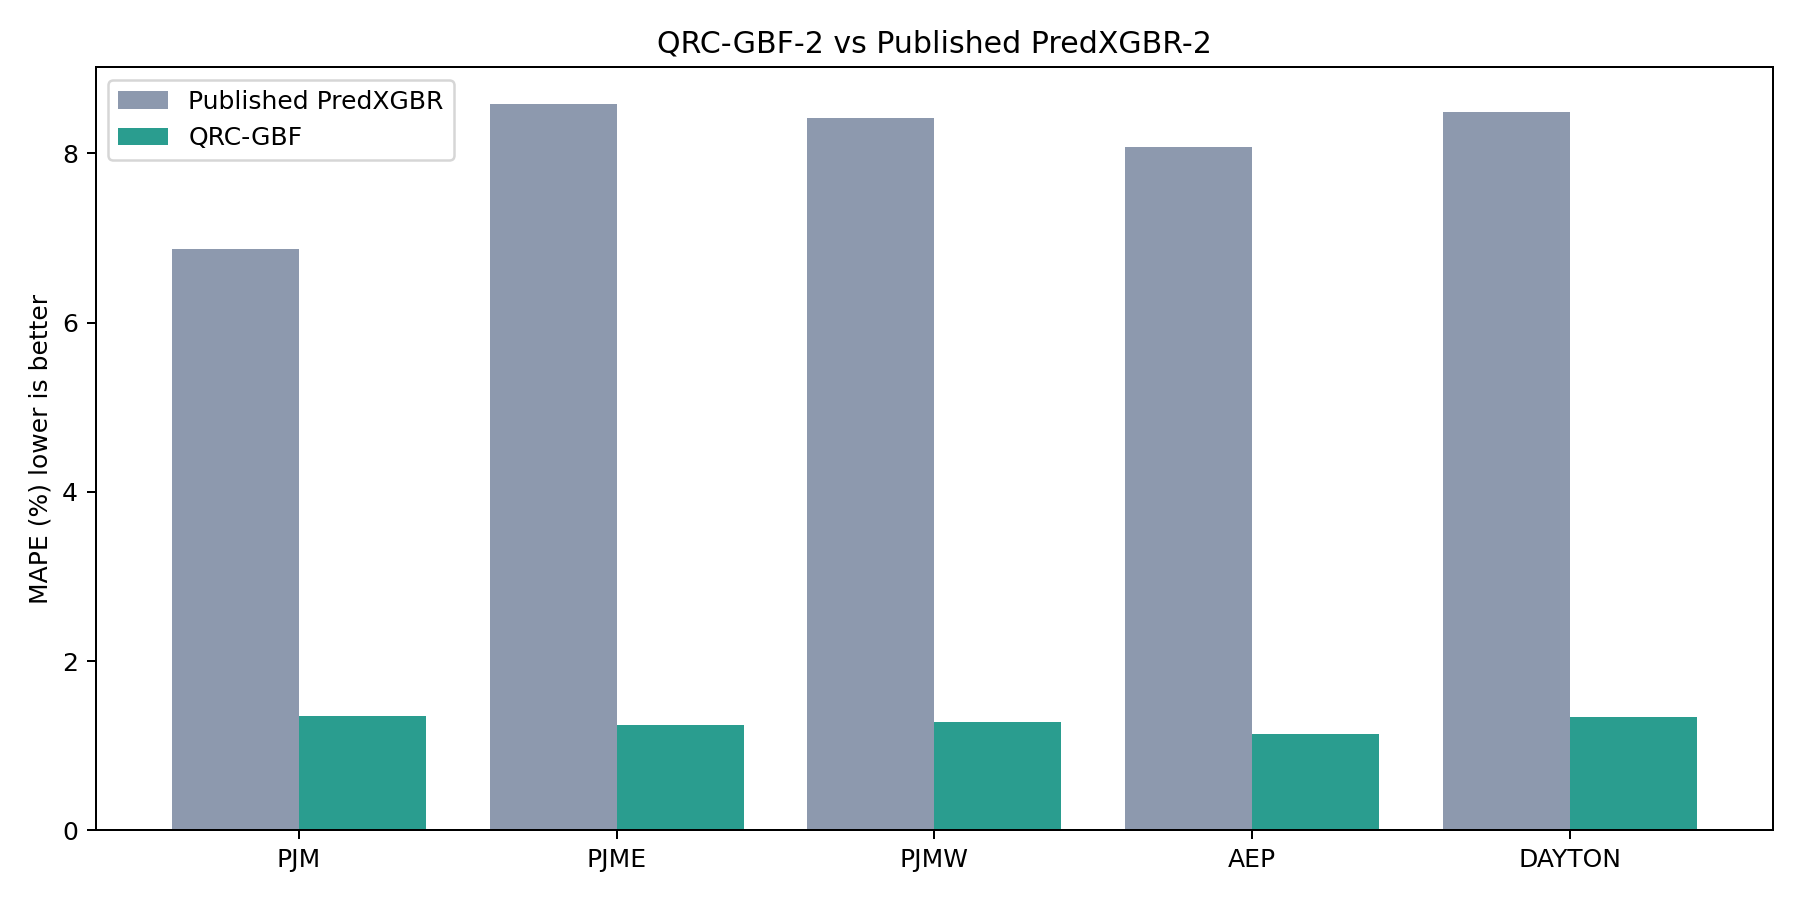
\includegraphics[width=0.9\linewidth]{figures/qrc_gbf_vs_predxgbr_model2.png}
\caption{External comparison: QRC-GBF-2 vs Published PredXGBR-2.}
\label{fig:model2_external}
\end{figure}

\subsection{Feature-Setting Comparison}
QRC-GBF-1 is better than QRC-GBF-2 on all five datasets. Local GBF-1 is also better than Local GBF-2 on all five datasets. This confirms the finding of the PredXGBR paper that short-term lag features are more effective for short-term forecasting.

\section{Ablation Study}
The internal ablation compares QRC-GBF against the corresponding local backbone. QRC-GBF-1 improves over Local GBF-1 on PJME, PJMW, and AEP, while Local GBF-1 remains slightly better on PJM and Dayton. QRC-GBF-2 improves over Local GBF-2 on all five datasets.

\begin{figure}[H]
\centering
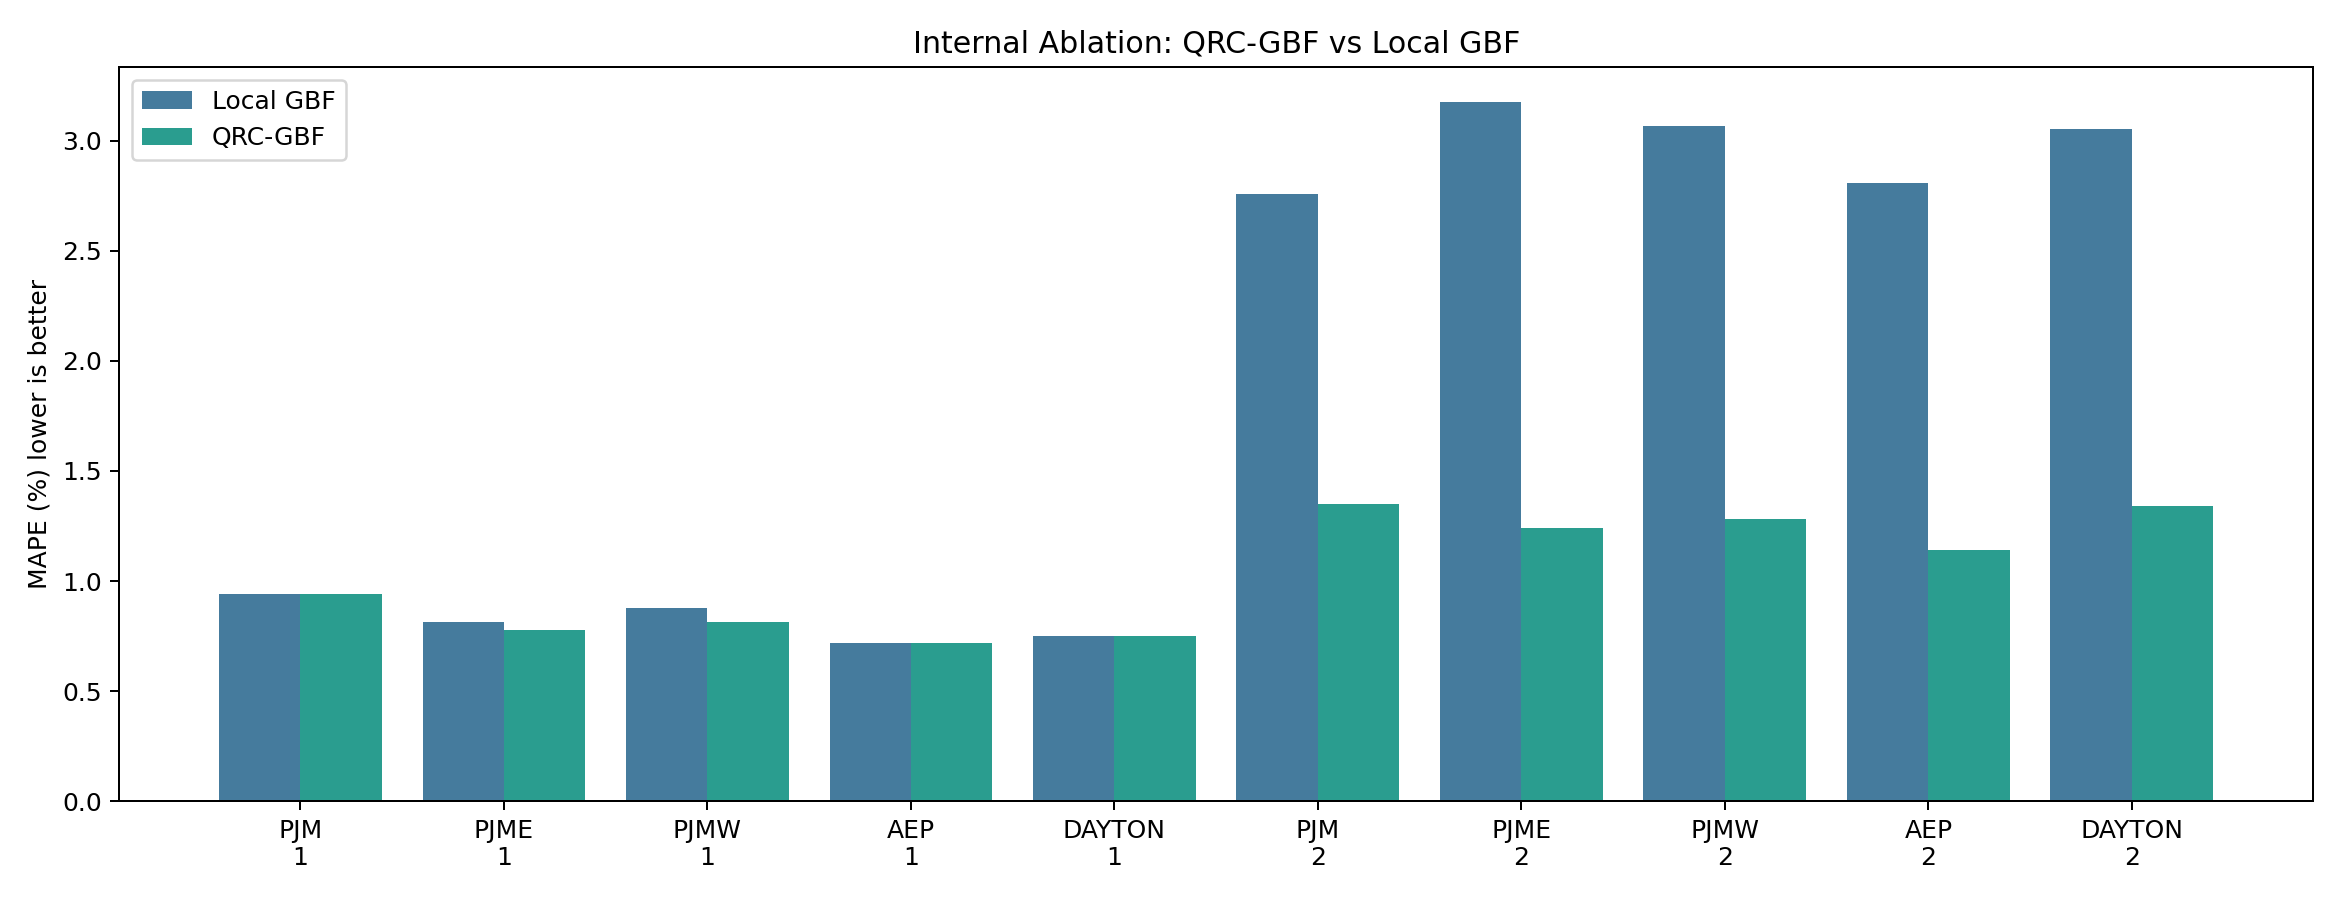
\includegraphics[width=0.98\linewidth]{figures/qrc_gbf_ablation_model1_model2.png}
\caption{Internal ablation: QRC-GBF versus Local GBF under Model 1 and Model 2 feature settings.}
\end{figure}

\section{Discussion}
The results show that the proposed method is strongest under the short-term feature setting. QRC-GBF-1 achieves the best overall MAPE across all datasets. QRC-GBF-2 still substantially improves over Published PredXGBR-2 and Local GBF-2, but it does not outperform QRC-GBF-1. This behavior is consistent with the short-term forecasting goal: recent load statistics provide more useful predictive information than broader long-term windows for one-step-ahead load forecasting.

The quantum residual branch should be interpreted carefully. QRC-GBF is a hybrid quantum machine-learning framework because it uses a VQC-based residual feature branch. However, the strongest improvements are produced by validation-selected residual correction, and the VQC branch is not claimed as universal quantum advantage.

\section{Limitations}
This work uses published PredXGBR values as external baselines and local GBF backbones as same-code ablations. Local GBF is not claimed to be an exact reproduction of PredXGBR because original implementation details are not fully matched. In addition, the VQC is evaluated using simulation rather than real quantum hardware. Future work should include stricter causal feature settings, larger VQC sweeps, more random seeds, and statistical significance tests.

\section{Conclusion}
This paper proposed QRC-GBF, a Quantum Residual Correction Gradient-Boosted Forecasting framework for short-term electrical load prediction. Following the PredXGBR Model 1/Model 2 structure, QRC-GBF-1 and QRC-GBF-2 were evaluated on PJM, PJME, PJMW, AEP, and Dayton datasets. QRC-GBF-1 outperformed Published PredXGBR-1 on all datasets, and QRC-GBF-2 outperformed Published PredXGBR-2 on all datasets. The strongest overall result was achieved by QRC-GBF-1, confirming that short-term lag features remain the most effective setting for short-term load forecasting.

\bibliographystyle{plain}
\bibliography{references}

\end{document}
